
We first motivate the need for a metamodel by outlining the requirements in disease modeling. We describe a basic and fundamental version of the metamodel that caters to the basic needs of epidemiological modeling and is attractive to experts with good understanding of compartmental epidemiological modeling, but not familiar with model-driven engineering practices. Next, we present how the proposed metamodel can be extended to accommodate the continuously evolving needs in epidemiological modeling. Building on the basic version, the extensions can provide additional support for automation and increase the expressiveness of basic models. Finally, we present the implementation of the metamodel with and without its extensions.

\subsection{Metamodel definition}

\subsubsection{Requirements}

Based on expert consultation, we have identified the following requirements for a basic metamodel for epidemics.
\begin{itemize}
    \item \emph{Support modeling of compartments}, to support basic compartmental models, such as the SEIR.
    \item \emph{Support runtime polymorphic compartment alternatives such as products \& groups}, to support stratification and other compartment composition tasks.
    \item \emph{Support modeling of flows}, to better model the mathematics behind transitions between compartments.
    \item \emph{Support runtime polymorphic flow alternatives such as batches, rates \& contacts}, to account not only for abstract flows, but also for those that best capture realistic scenarios.
\end{itemize}
The aforementioned requirements also include the inherent requirements for the composability of models and model components, as well as the polymorphism of flows to allow for transitions between any kind of compartments and their compositions.

\subsubsection{The basic metamodel}

\texttt{EpiMDE-model} is a metamodel designed for immediate usability by epidemiologists, using familiar concepts from compartmental modeling. The core of \texttt{EpiMDE-model} consists of \textbf{Compartments} connected via \textbf{Flows}. Each Compartment has a name and an initial population attribute, and contains a list of its outgoing flows. \texttt{EpiMDE-model} supports two types of flows: \textit{RateFlow} for time-based transitions (e.g., progression from exposed to infectious), and \textit{ContactFlow} for disease transmission through contact between susceptible and infectious individuals.

A key feature of \texttt{EpiMDE-model} is its support for \textbf{population stratification}. Rather than requiring modelers to create separate compartments for each stratum (which would result in an explosion of compartments and flows), \texttt{EpiMDE-model} provides explicit stratification mechanisms.

\paragraph{Stratification Mechanism}

Stratification in \texttt{EpiMDE-model} works through a three-level hierarchy that separates stratification dimensions from disease compartments:

\begin{enumerate}
    \item \textbf{Groups define stratification dimensions}: A \textit{Group} represents a single stratification dimension with multiple values. For example, an age Group might contain values [0-19, 20-64, 65+], while a sex Group contains [Male, Female]. Each Group is a container of compartment strata that share a common characteristic.

    \item \textbf{Products combine multiple dimensions}: A \textit{Product} takes multiple Groups as input and computes their Cartesian product, generating all possible combinations of strata. For example, if an age Group has 3 values and a location Group has 2 values, their Product generates $3 \times 2 = 6$ unique stratum combinations: (0-19, Location-A), (0-19, Location-B), (20-64, Location-A), (20-64, Location-B), (65+, Location-A), (65+, Location-B).

    \item \textbf{Compartments reference Products for stratification}: Disease compartments (S, E, I, R) reference a Product to indicate they should be stratified. When a compartment references a Product with 6 strata, the metamodel automatically generates 6 physical compartments (one for each stratum) from that single logical compartment definition. This expansion is transparent to the modeler---they define the stratification structure once and reference it, rather than manually creating dozens or hundreds of stratified compartments.
\end{enumerate}

For example, stratifying an SEIR model by both age (3 groups) and location (2 groups) creates $4 \times 3 \times 2 = 24$ physical compartments from just 4 logical compartments in the model. The modeler creates:
\begin{itemize}
    \item One age Group with 3 values
    \item One location Group with 2 values
    \item One Product combining these Groups (6 strata)
    \item Four compartments (S, E, I, R) each referencing the Product
\end{itemize}
At model instantiation time, the platform automatically expands this to 24 physical compartments with appropriate labeling (e.g., S-[0-19]-[Location-A], S-[0-19]-[Location-B], etc.). Flows defined between logical compartments are similarly expanded to connect the corresponding physical compartments, with parameters automatically replicated or stratified as specified by the modeler.

An important design decision in \texttt{EpiMDE-model} is that Groups and Products form a \textbf{separate subgraph} from the Compartment-Flow graph structure. This is intentional: Groups and Products define the \emph{dimensions of stratification}, which are orthogonal to the \emph{epidemiological dynamics} represented by compartments and flows. This separation maintains conceptual clarity. The stratification structure (``how should we divide the population?'') is defined independently from the disease progression structure (``how does the disease spread?''). Compartments reference Products via associations to indicate which stratification applies to them, but Groups and Products themselves do not participate in the flow network. This design also enables stratification definitions to be reused across multiple models within the same modeling project.

\texttt{EpiMDE-model} also includes \textbf{external population dynamics}. An \textit{ExternalSource} represents population inflow (e.g., births entering the susceptible compartment, or immigration), while an \textit{ExternalSink} attached to a compartment represents natural mortality outflow or emigration. Finally, \textbf{heterogeneous rates} across strata are supported via \textit{StratumSpecificRate}, which allows modelers to specify different rate values for different population segments, either as absolute rates or as multipliers applied to a base rate.

There are several benefits to \texttt{EpiMDE-model}. First, the conceptualization is \textbf{familiar} to epidemiologists. Compartments, flows, and stratification are standard concepts in the field, making \texttt{EpiMDE-model} immediately accessible without requiring MDE expertise. Second, \texttt{EpiMDE-model} provides \textbf{explicit stratification support} through Groups and Products, avoiding the manual explosion of compartments and flows that would otherwise be required. This significantly reduces modeling effort while maintaining clarity. Third, all elements are \textbf{domain-specific}. There are no abstract wrappers or technical constructs unrelated to epidemiology. Finally, the models are \textbf{transparent}. What the modeler creates directly represents the epidemiological structure without hidden transformations.

\paragraph{Design Rationale for Accessibility}
The design of \texttt{EpiMDE-model} was driven by collaboration with epidemiologists who emphasized the need for a tool that does not require software engineering or MDE expertise. Traditional compartmental modeling tools (e.g., STEM, IDM-CMS) often require extensive manual coding or complex configuration files, which are error-prone and time-consuming. \texttt{EpiMDE-model} addresses this through three key design decisions. First, \textit{graphical modeling} allows epidemiologists to construct models visually using concepts they already understand, rather than writing hundreds of lines of equations by hand. Second, \textit{automatic equation generation} eliminates the need to manually derive and implement differential equations, a process that is both tedious and prone to transcription errors, especially for stratified models. Third, \textit{built-in validation} through metamodel constraints prevents common modeling errors (e.g., missing flows, inconsistent stratification) at design time rather than discovery during simulation. Our case studies (Sections~\ref{sec:study}) demonstrate that epidemiologists can replicate published models using \texttt{EpiMDE-model} with minimal training, validating these design choices.

While \texttt{EpiMDE-model} prioritizes accessibility and usability, it has trade-offs in terms of \textbf{advanced automation} and \textbf{extensibility}. \texttt{EpiMDE-model} provides the essential features needed for most compartmental models, but lacks extension mechanisms for modeling novel disease dynamics or advanced interventions that may emerge during research. The metamodel is intentionally kept simple and fixed to minimize the learning curve, which means it cannot be easily adapted to incorporate new modeling paradigms beyond compartments, flows, and stratification. These limitations motivated the development of the extensible metamodel, which provides wrapper-based abstractions and extension points for advanced users. The expectation is that modelers will start with \texttt{EpiMDE-model} for its simplicity and accessibility, and may transition to the extensible version as their modeling needs become more sophisticated.

\subsubsection{Metamodel extensibility}

In order to account for more specific cases, to allow for modeling of a greater variety of diseases and accommodate the evolution of a disease, our metamodel can be extended. To differentiate between the basic metamodel and its extensions, we talk about compartments and flows, in the case of the former, and about physical compartments and physical flows, in the case of the latter, which can be perceived as specializations of the abstract compartments and flows, as will be explained later. The extensions, in order to provide adequate and manageable complexity, are governed by the following requirements.
\begin{itemize}
    \item Compartments must:
    \begin{itemize}
        \item provide their sources and sinks, i.e., other compartments with transitions to and from this compartment.
        \item produce their physical compartments and equations.
    \end{itemize}
    \item Physical compartments must:
    \begin{itemize}
        \item be represented as lists of labels of the compartments, which they are composed of.
        \item contain each of the labels of the compartments used during their generation.
    \end{itemize}
    \item Flows must:
    \begin{itemize}
        \item support parameterization according to patterns defined by the metamodel.
    \end{itemize}
    \item Physical flows must:
    \begin{itemize}
        \item reference a source and a sink physical compartment.
        \item use a lisp-like syntax for their equation.
    \end{itemize}
\end{itemize}



In the proposed metamodel, base compartments can be extended to include groups, products and basic reproduction number compartments, while base flows can be extended to represent cross-rates and other complex flows.

\paragraph{Groups}

Consider a representation of an SIR model, a simplified version of the SEIR model without an ``Exposed'' compartment, as an array of compartments: [$S$, $I$, $R$]. In our metamodel, this array is an element type called a \textit{group}. Groups are composed of compartments and flows. Groups can be used in place of a unit compartment to provide more details. For example, a three-element SIR model could be made into a four-element SIR model  which accounts for symptoms using a group for $I$ instead of a unit compartment: [$S$, $I$=[$I_{Asymptomatic}$, $I_{Symptomatic}$], $R$]. Groups enable graph vertex substitution\cite{PREVITE_1998}. By providing groups with sources and sinks, it is possible to connect them to other compartments appropriately. For example, it could be specified that $I_{Asymptomatic}$ is a source and $I_{Symptomatic}$ is a sink. Doing so means that a flow from $S$ to $I$ would then point only to $I_{Asymptomatic}$ while a flow from $I$ to $R$ would point only from $I_{Symptomatic}$.

Simulation artifacts produced by our models must provide a list of compartments and equations. Compartments such as groups will rely on the artifacts produced by their children. Our models are tree structures, while the produced artifacts are a flattened representation. Generated compartments will be referred to as physical compartments, as it corresponds to the representation used for simulation.
The same applies to flows.

\paragraph{Products}
In order to represent model stratification, the simplest approach is to make use of a product compartment type. Products perform a Cartesian product of their children. A product's children are its dimensions. Typically, Cartesian products produce lists of lists of elements from lists of lists of elements. For example, consider two groups $A$ and $B$ with children $1$, $2$ and $3$, $4$ respectively. One intuitive way to to represent this physically is by concatenating the lables, like [$A1B3$, $A1B4$, $A2B3$, $A2B4$], but this may become too complex and does not facilitate the mathematical simulation of the model. Instead, our model produces lists of labels instead of concatenated strings. Thus, the above product would be represented as [[$A$, $1$, $B$, $3$], [$A$, $1$, $B$, $4$], [$A$, $2$, $B$, $3$], [$A$, $2$, $B$, $4$]]. This preserves the identity of the original labels and is closer to the mathematical model of a Cartesian product. Lists also make it simple to verify if two physical compartments share the same set of labels for example, which is important since it would be a modeling error.

\paragraph{Basic Reproduction Number Compartment}

A fundamental parameter of epidemiological models is the basic reproduction number or $R_0$ (pronounced ``R nought''), which represents the the expected number of cases directly generated by one case in a population where all individuals are susceptible to infection. Different diseases or even different variants of the same disease can have different $R_0$, which is an important fact for simulations. $R_0$ does not correspond to any inherent property of the studied disease, but it is rather estimated mathematically based on the properties of the population.

The $R_0$ extension of our metamodel is a type of compartment composed of one child compartment, a compartmental model which we want to evaluate the $R_0$ for. The simulation artifacts produced by this compartment will duplicate the model in two copies, one containing the originally infectious or exposed population, and one containing the susceptible population. By disabling infectiousness of the second copy, all infections are caused by originally infected people, which we can divide by the number of infectious people in the scenario, enabling the automatic calculation of the $R_0$.

There are many implementations of this extension which do not break our modeling assumptions and do not require additional requirements. That is to say, creating two copies and disabling the exposure flow for one of the copies is possible given our proposed metamodel. This extension is particularly useful as it is easily reusable and serves a very concrete purpose. While it models a moderately complex extension, it does not add any extra requirements to our metamodel, further demonstrating its flexibility and extensibility.

\paragraph{Basic Flows}
Typical epidemiological models make use of rates, batches and contacts, which are represented as mathematical equations in the final model. The three types have some structural and functional similarities. It is also possible that other more complex flows may have to be modeled in the future. For this reason, we propose an abstraction of the basic flows to allow for polymorphism and future extensibility. 

Our solution is to represent equations in a Lisp-like syntax, enabling arbitrary mathematical expressions that are simple to parse. A basic flow has a source, a destination and a Lisp-like equation. We would represent the contact in a typical SEIR model as \texttt{\{from: [S], to: [E], equation: (sumproduct [S] [I])\}}, omitting parameters for simplicity. The sumproduct is essentially a dot product, since \texttt{[S]} and \texttt{[I]} can be stratified compartments. The brackets are used to denote compartments, which are identified by their associated lables. In the event where \texttt{[S]} or \texttt{[I]} denotes multiple compartments, such as each age group, this evaluates to a vector of population values. The use of Lisp-like makes it simple to parse nested equations, as it does not require operator precedence, unlike regular mathematical expressions.

Most equations require at least one constant to calibrate them. For example, let us consider two parameters of a contact, namely the susceptibility of the source compartment and the contagiousness of the contact compartment. Including these parameters in the equation produces \texttt{(sumproduct (* (parameter susceptibility [S]) [S]) (* (parameter infectiousness [I]) [I]))}.
Similarly to the stratification of the populations, if \texttt{[I]} is stratified along age, parameters relying on \texttt{[I]} are also stratified. This means that \texttt{(parameter infectiousness [I])} has the same number of elements as \texttt{[I]} and so does their product "*", which is not a dot product but rather a Hadamard product, accepting an arbitrary number of vectors of the same dimension.

Knowing where to place the parameters in the equation requires knowledge about what the purpose of the parameter is. For this to be possible, since a metamodeler does not know the intent of every modeler, the metamodel needs to abstract parameterization according to frequently used patterns. Here we propose five patterns which are available for rates and contacts.
\begin{enumerate}
    \item \textit{Single-value} is used to multiply all equations generated from a flow with the same value. The multiplication factors is assigned to all instances of the flow depending on the stratifications of the compartments. For example, in the case of hospitalization in the ICU, if a flow from $ICU$ to $post-ICU$ has a rate of $1/21$ and the there are 5 age stratifications and 2 sex stratifications, all 10 flow instances will be multiplied with the same rate.
    \item \textit{Multi-valued (source)} is used to multiply each generated equation with a specific value. Similar to single-value, all flow instances will be multiplied, but this time with a unique rate for each flow.
    \item \textit{Multi-valued (sink)} is used to weigh the outputs of an equation which points to multiple compartments. For example, if a flow from one compartment goes to multiple other compartments, this parameter is used to weight differently the outgoing flows from the source compartment. Typically, the sum of the sink parameters will be 1 as to simplify reasoning about the overall flow's throughput and read the values like probabilities.
    \item \textit{Multi-valued (contact)} is used to multiply each contact population with a specific value. for example to provide an $infectiousness$ parameter to a contact equation to weigh each infectious compartment:
    Equation $S_i * sum(I)$ becomes $S_i * sum(infectiousness * I)$.
    \item \textit{Multi-valued (contact \& source)} is used to multiply each contact population with a specific value for each source. An example of this pattern can be applied in the case of a contact-matrix, built from a large population study. A given value in the matrix describes how many daily contacts an average person of a certain age group has with another group. A row describes the contacts of a certain age group with all the others, depending on the number of stratifications. The strength of the exposure is weighed with the sum of the element wise multiplication of the appropriate row of the contact matrix and the populations of I compartments. Formally, equation $S_i * sum(I)$ becomes $S_i * sum(contact_i * I)$. In the multi-valued (contact) example, the infectiousness values are shared. Here, each equation uses the contact matrix row for its population.
\end{enumerate}


\paragraph{Complex Flows}

Depending on the disease and context, users will want to make use of more complex equations to represent some phenomena. One such example is the modeling of HIV. Being a sexually transmitted disease, it poses modeling concerns that do not appear in most other infectious disease models. Due to its longevity (more than 40 years recognized as an epidemic), modeling HIV is particularly difficult as it is important to account for births as well as relationships. Studies also show that modeling relationship behaviours is equally important. For example, depending on social context and available treatments, women can contract HIV at a greater rate than men due to abusive relationships \cite{Woolfork2020-nt}. 

In order to model relationships, we require new types of flows. The problem at hand is to model relationship creation and, when they come to an end, remove relationship status of both individuals at the same time. Undoing relationships correctly is simple. For example, consider a $male-female-relationship$ compartment with a rate to compartment $single-male$ as well as a rate to $single-female$. Assuming both rates use the same equation, relationships will break evenly, placing the same amount of men and women back to their respective single compartment.

The problem lies in producing relationships given a population of men and women. Making use of batches with set amounts is a solution, but it is not as natural as using rates. Let us consider the following heterosexual relationship example. Using two rates with the same constant, one from male and one from female, but one making use of the male population and the other the female, we end up with an invalid model. Even a slight difference between the male and female population would lead to a disparity where more or fewer men are entering heterosexual relationships than women and our model would not make sense. To solve this problem, we introduce cross-rates, a new type of flow which proves useful in different contexts and helps verify the validity of our current requirements.

\paragraph{Cross-Rates}

This new type of flow is similar to a rate but does not use its source population in the calculation, making use of another compartment's population instead. Cross-rates describe a flow from compartments $A$ to $B$ with equation $constant$ * population of $C$, where $C$ is any of the two compartments. In the context of modeling relationships, cross-rates can be used as flows from $Male$ and $Female$ to $Relationship$ with equation $constant$ * population of $Group[Male, Female]$.

\subsection{Metamodel implementation}

Having detailed our set of types and their use for epidemiological modeling, we now provide an implementation, using the Eclipse Modeling Framework (EMF)~\cite{steinberg2008emf}, for our metamodel. The full metamodel is composed of the base metamodel and selected extensions, each of which has a separate diagram, being a different modeling project. The metamodel will first be presented graphically, then some programming implementation details will be included.

\subsubsection{EMF Wrappers}

EMF supports metamodel extensibility in a limiting manner. For clarity, let us consider the following example, where we have a metamodel $M$ with extensions $MBox$ and $MPen$.
\begin{itemize}
    \item Let $M$ declare an abstract class $Object$.
    \item Let $M$ declare a concrete type $Bag$ inheriting from $Object$.
    \item Let $MBox$ declare a concrete type $Box$ inheriting from $Object$.
    \item Let $MPen$ declare a concrete type $Pen$ inheriting from $Object$.
    \item Let both $Bag$ and $Box$ be composed of $0..*$ $Objects$.
\end{itemize}

The expected behaviour is for both $Bag$ and $Box$ to be allowed to contain $Pens$, but this is not the observed behaviour. The extension mechanism of EMF is for extensions of $M$ such as $MBox$ and $MPen$ to add their $Objects$ as alternatives for members of $Bag$. Since $MPen$ and $MBox$ are unaware of each other, $Boxes$ cannot contain $Pens$.

The solution to this is to introduce \textit{wrappers}. By introducing a wrapper such as $ObjectWrapper$ in $M$, a concrete type composed of exactly 1 $Object$, the problem can be solved. $Bags$ and $Boxes$ will now be composed of $0..*$ $ObjectWrappers$. The extension mechanism now allows for $MBox$ and $MPen$ to interact. $Boxes$ may contain an $ObjectWrapper$ from $M$ which was extended by $MPen$, allowing for $Boxes$ to contain $Pens$. In a similar manner, wrappers are used in our metamodels to allow products and groups to contain each other. The use of wrapper will be present in types making use of composition of compartments or flows.

\subsubsection{Metamodel Graphical Implementation}

Figure~\ref{fig:compartmental_classdiagram} shows the complete UML class diagram of the \texttt{EpiMDE-model} metamodel, illustrating all classes, attributes, and relationships. This provides an overview of the metamodel structure, showing how Compartments, Flows (RateFlow and ContactFlow), ExternalSources, ExternalSinks, stratification elements (Groups and Products), and parameters are related. In the following paragraphs, we examine specific aspects of this metamodel in detail.

\begin{figure}[t]
    \centering
    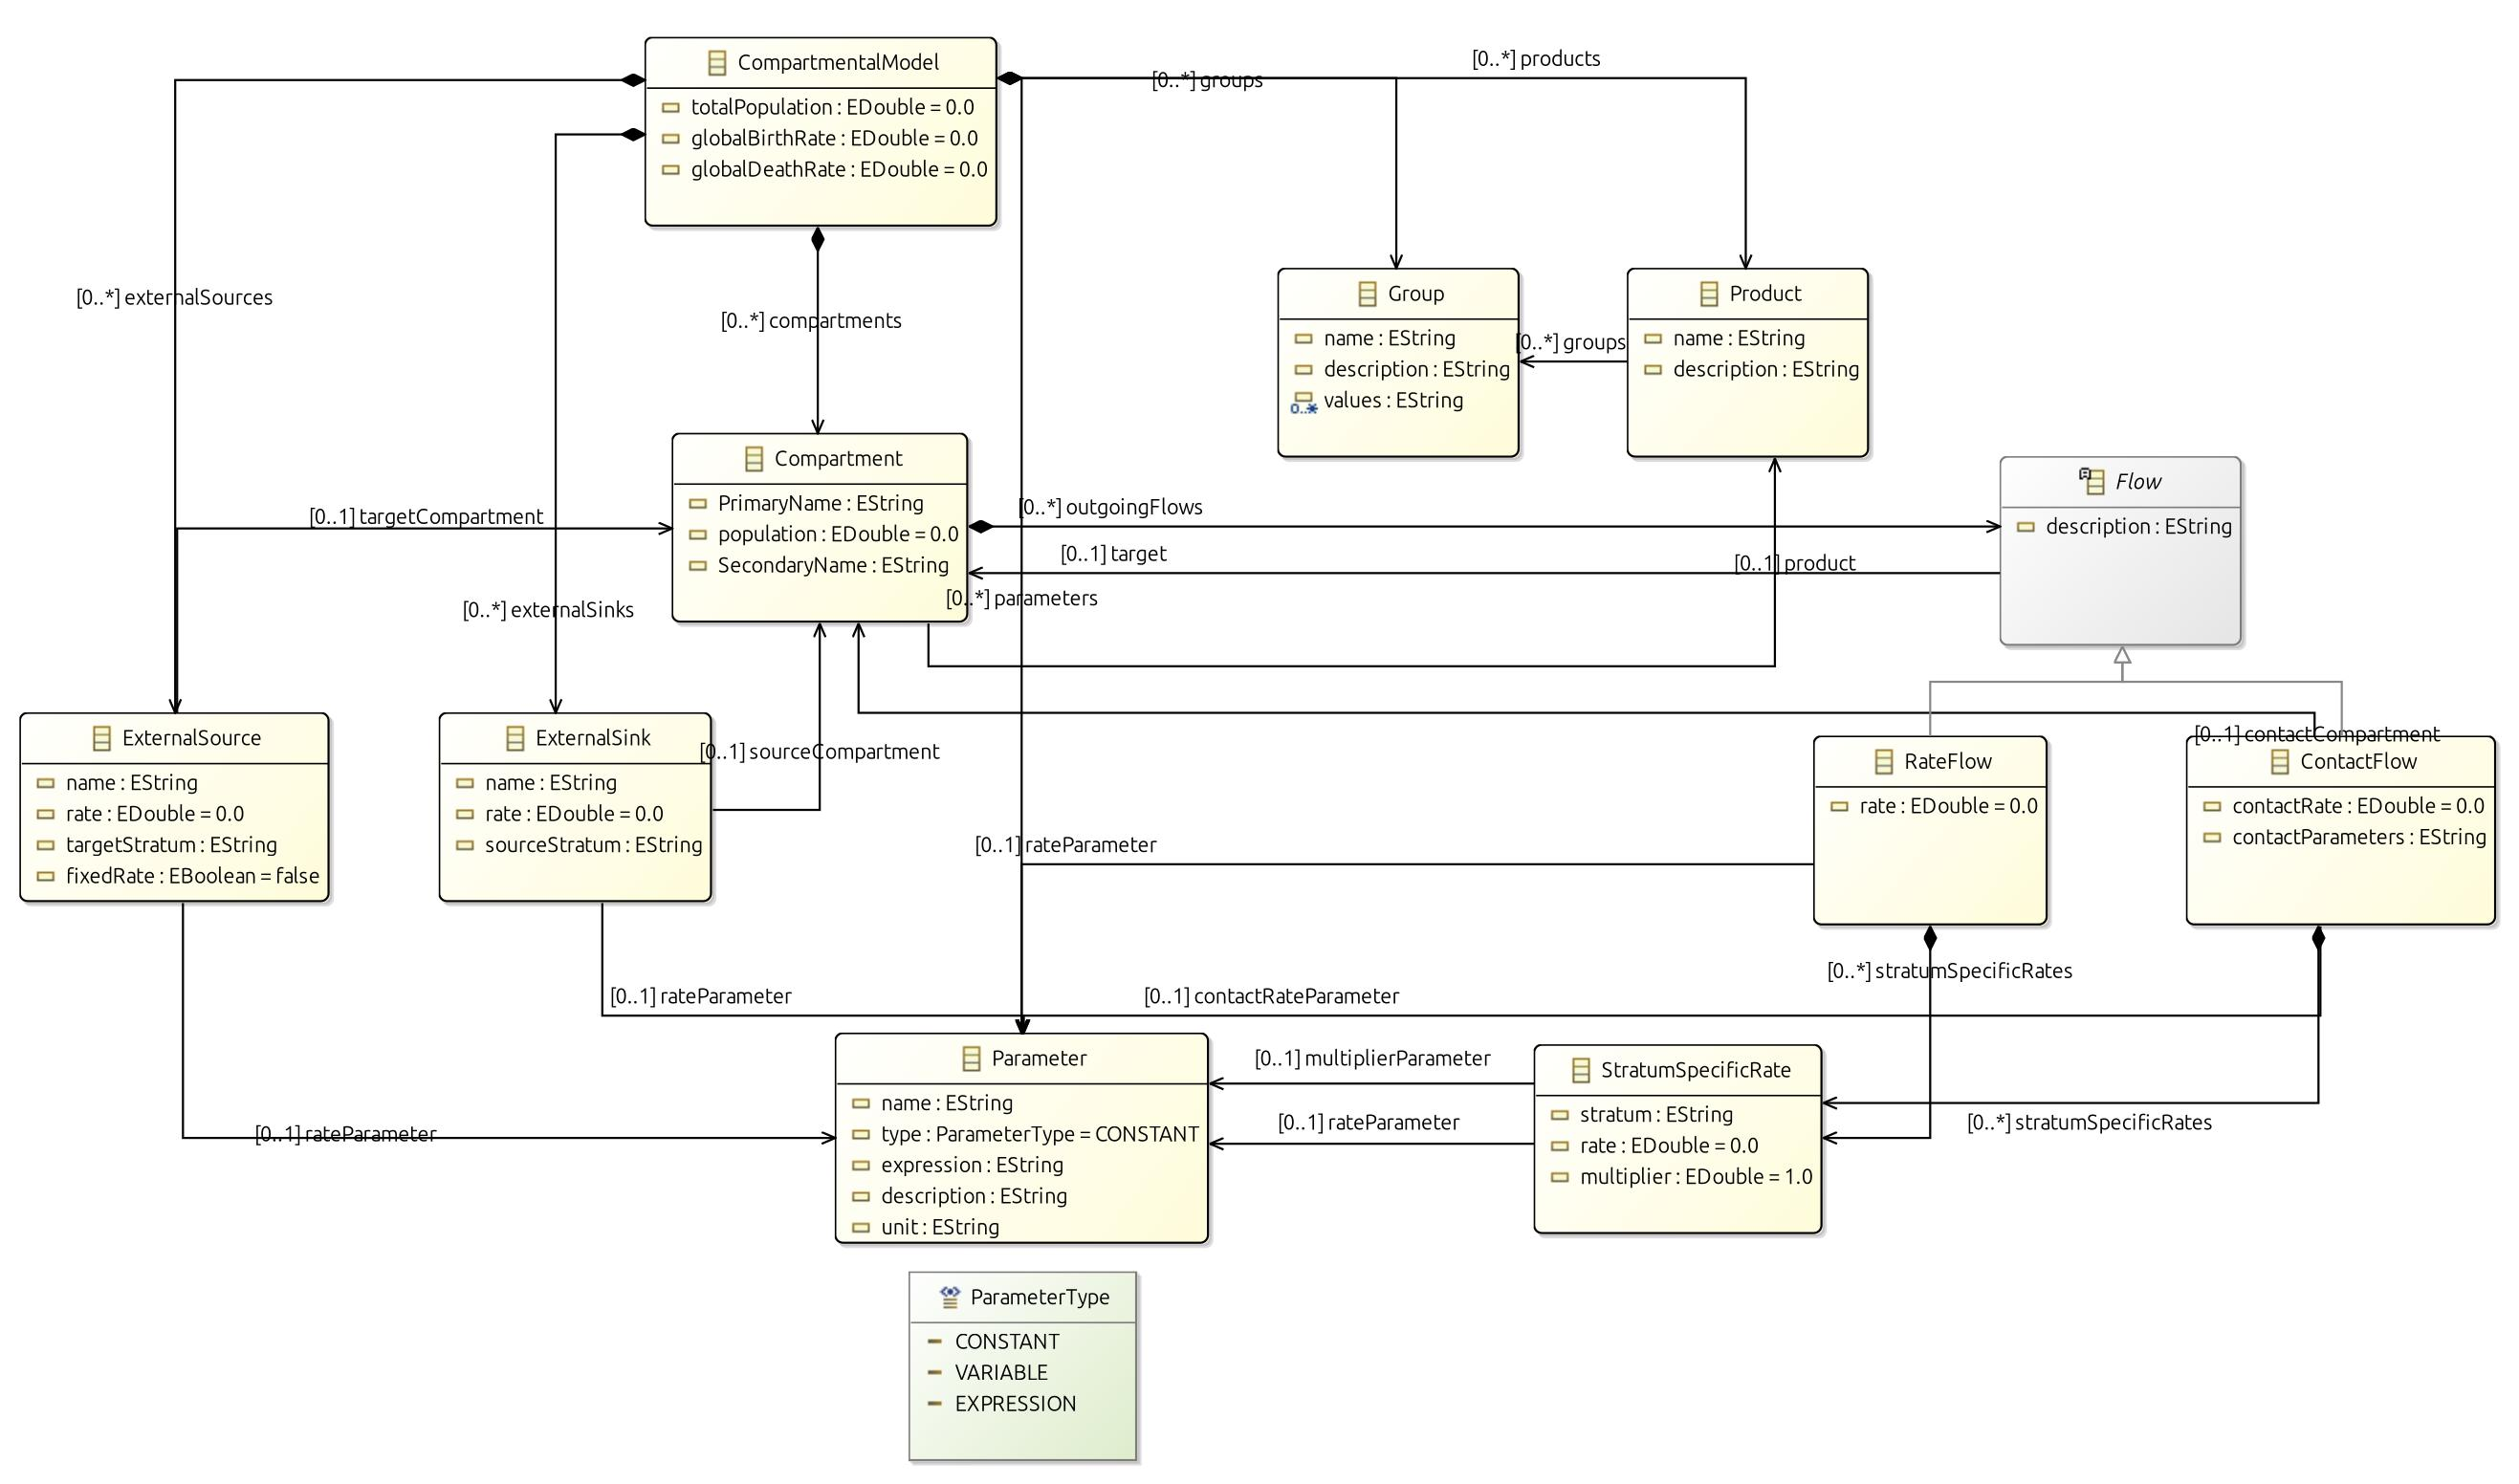
\includegraphics[width=\linewidth]{Figures/compartmentalmodel_classdiagram.jpg}
    \caption{The structure of the \texttt{EpiMDE-model} metamodel. The metamodel defines compartments, groups and products, as well as flows and simulation parameters.}
    \label{fig:compartmental_classdiagram}
\end{figure}

\texttt{EpiMDE-model} is using Sirius~\cite{viyovic2014sirius} to provide a graphical editor for its models and metamodels. The base metamodel declares the top level type $Epidemic$ as well as the $Compartment$ and $Flow$ types. An epidemic is composed of a single compartment, either a product or a group. The base $Compartment$ type is a unitary compartment class which generates a single physical compartment from its labels.



\paragraph{Groups and Products}

The group metamodel extension describes groups and products. A group is composed of any number of compartments and flows, and it extends the $Compartment$ class. Groups also reference some of their compartments as either $source$, $sink$, both or neither. Not all constraints can be seen in the metamodel diagram. For example, though a group could reference any compartment as its sink or source, the referenced compartments must be its direct children. Products are identical in structure to groups, except for the sources and sinks. Products derive their sources and sinks from the product of the sources and sinks of their children. Figure~\ref{fig:compartmental_classdiagram} shows the simplified implementation of Groups and Products, where stratification is represented directly without the compartment wrapper mechanism used in the extensible version for dynamic composition.



%\paragraph{Product}

%Figure \ref{fig:product_mm_graph} describes the product metamodel extension. 


%\begin{figure}[t]
%    \centering
%    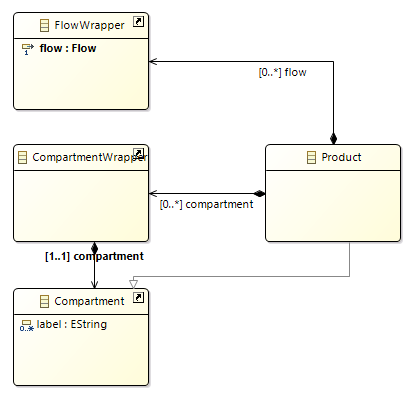
\includegraphics[width=0.6\linewidth]{Figures/product_mm_graph.png}
%    \caption{Product Metamodel}
%    \label{fig:product_mm_graph}
%\end{figure}

%Products are identical in structure to groups, except for the sources and sinks.
%Products derive their sources and sinks from the product of the sources and sinks of their children.
%The ability to place flows in products was not discussed and is not particularly important, it can be ignored.
%The idea is that a user could place an existing SEIR model in a product and add a flow from R to S, forming a typical SEIRS model.
%This could be done in groups too, not just products.
%Peeking inside a group from the outside is not necessarily good or bad, but is up for debate in future versions.


\paragraph{Basic Flows}
The basic flows extension provides the three basic types of flows: rates, batches and contacts. By making use of the class $FromToFlow$ in the hierarchy some functionalities common to all three flows are easily shared. Figure~\ref{fig:compartmental_classdiagram} shows a simplified subset of this extension, including $RateFlow$ and $ContactFlow$ types, which cover the most common epidemiological modeling scenarios, while the extensible version additionally includes batch flows for more specialized use cases.



\subsubsection{From metamodel extensions to models}

\begin{algorithm}[t]
\caption{Produce Physical Compartments of Group}
\label{alg:group}
\begin{algorithmic}
\Procedure{GetPhysicalCompartments}{}
\For{$wrapper \in this.getCompartment()$}
    \State $cmpt \gets wrapper.getCompartment()$ 
    \For{$pc \in cmpt.getPhysicalCompartments()$}
        \State $\textbf{yield} \: this.prependSelf(pc)$
    \EndFor
\EndFor
\EndProcedure
\end{algorithmic}
\end{algorithm}

\begin{algorithm}[t]
\caption{Produce Physical Compartments of Product}
\label{alg:product}
\begin{algorithmic}
\Procedure{GetPhysicalCompartments}{}
\State $\textbf{alias} \: PC \gets PhysicalCompartment$
\State $List$<$List$<$PC$\text{>}\text{>} $ \: dimensions \gets []$
\For{$wrapper \in this.getCompartment()$}
    \State $cmpt \gets wrapper.getCompartment()$
    \State $List$<$PC$>$ \: dim \gets cmpt.getPhysicalCompartments()$
    \State $dimensions.add(dimn)$
\EndFor
\State $List$<$List$<$PC$\text{>}\text{>} $\:prod \gets CartesianProduct(dimensions)$
\For{$List$<$PC$>$ \: pcs \in prod$}
    \State $PC \: pc \gets join(pcs)$
    \State $\textbf{yield} \: this.prependSelf(pc)$
\EndFor
\EndProcedure
\end{algorithmic}
\end{algorithm}

Given the extension mechanisms discussed previously, it becomes evident that the task of creating a model from the proposed metamodel is not a straightforward process. Normally, a metamodel would serve as the DSL that would guide the creation of models; it informs the modeler of what elements are available, how they can be connected, what properties they can have and what constraints govern their structure and relations. As we have mentioned, the metamodel extensions we propose here are based on abstract notions that before being used in concrete models they have to become concrete or ``physical'' as we call the resulting components. Thankfully, this process, which we will discuss here, is hidden from the modeler, who only sees the resulting DSL.

The processes for generating the physical components for $Groups$ and $Products$ are described in java-like pseudo code in Algorithms~\ref{alg:group} and~\ref{alg:product} respectively. Note that all $.getCompartment()$ methods are automatically generated by EMF from the compositions in the UML diagram being named $compartment$. The version for compartment wrappers returns a compartment while the group and product versions return $EList$ of compartment wrappers. $prependSelf$ is a utility to add the labels of the current compartment at the beginning of the labels list of the produced physical compartments.

\paragraph{Algorithm Explanation}

\textbf{Algorithm~\ref{alg:group} (Group Physical Compartments Generation)} transforms a Group's logical structure into its physical representation through a flattening process. The algorithm operates as follows:
\begin{enumerate}
    \item \textbf{Iterate through child compartments} (lines 2-3): For each compartment wrapper contained in the Group, extract the underlying compartment. This handles the EMF wrapper mechanism described in Section~\ref{sec:metamodel}.
    \item \textbf{Recursively expand children} (lines 4-5): Call $getPhysicalCompartments()$ on each child compartment. This recursive call handles nested Groups and Products, ensuring full expansion regardless of hierarchy depth.
    \item \textbf{Prepend Group label} (line 5): For each physical compartment produced by a child, prepend the current Group's label to create a hierarchical label path. For example, if Group ``Age'' contains compartment ``Child'', the physical compartment becomes ``Age-Child''.
    \item \textbf{Yield results} (line 5): Return each labeled physical compartment one at a time, enabling lazy evaluation for large stratifications.
\end{enumerate}
The algorithm's key insight is that Groups simply flatten their children while maintaining hierarchical labeling. If a Group contains 3 child compartments, it produces 3 physical compartments with prepended labels.

\textbf{Algorithm~\ref{alg:product} (Product Physical Compartments Generation)} implements Cartesian product logic to generate all stratum combinations. The algorithm proceeds as follows:
\begin{enumerate}
    \item \textbf{Collect dimensions} (lines 2-6): Iterate through all child compartments (each representing a stratification dimension), recursively expand each to physical compartments, and store the result as a dimension. For example, an age Group with 3 values and a sex Group with 2 values create two dimensions: $[[Age_1, Age_2, Age_3], [Sex_1, Sex_2]]$.
    \item \textbf{Compute Cartesian product} (line 7): Apply the mathematical Cartesian product operation to the list of dimensions. This generates all possible combinations: if dimensions have sizes $[n_1, n_2, ..., n_k]$, the product produces $n_1 \times n_2 \times ... \times n_k$ combinations. For the age-sex example, this produces 6 combinations: $(Age_1, Sex_1), (Age_1, Sex_2), (Age_2, Sex_1), ..., (Age_3, Sex_2)$.
    \item \textbf{Join labels} (lines 8-9): For each combination (a list of physical compartments), merge their labels into a single physical compartment. For example, $(Age_{20-64}, Location_A)$ becomes a single physical compartment with label $[Age, 20-64, Location, A]$.
    \item \textbf{Prepend Product label} (line 9): Add the Product's own label to the beginning of the merged label list, creating a complete hierarchical path.
    \item \textbf{Yield results} (line 9): Return each product physical compartment, enabling lazy evaluation.
\end{enumerate}
The algorithm's complexity is $O(n_1 \times n_2 \times ... \times n_k)$ where $n_i$ is the size of dimension $i$, which is inherent to the Cartesian product operation. In practice, Products typically have 2-3 dimensions with 2-5 values each, resulting in manageable expansion (e.g., $3 \times 2 = 6$ or $4 \times 3 \times 2 = 24$ physical compartments).



The algorithms to generate sources and sinks are quite similar. Groups gather the source physical compartments of its source compartments, while products produce the Cartesian product of the source physical compartments of their children. The algorithms used to gather equations are nearly identical. Algorithms used by flows to produce their physical representations rely on the parameterization patterns that were presented before.